% !TEX root = paper.tex

\subsection{Intuition}
Given the features extracted from the physiological process, it seems plausible to perform any classification algorithm for blood glucose level prediction. Nonetheless, this plug-and-play approach will neglect important information from (1) dynamics of the process, and (2) inter-user similarity among same group of participants. Traditionally, various sequential classification methods[], e.g., hidden Markov model (HMM), recurrent neural networks (RNN), and dynamic conditional random fields (CRF), are used to capture the temporal correlation of the input feature. The inter process correlations are often times incorporated with the so-called multi-task learning approaches[], which learns processes (or tasks) in parallel to improve classification or to reduce the data sample requirement. 

In this paper, a novel machine learning paradigm, namely Multi-division deep-dynamic RNN (Md$^3$RNN), is proposed. To include the the aforementioned information sources in an unified framework, we develop two key ideas that extend the classical RNN. Firstly, the single hidden layer in RNN is replaced with several deep stacked layers. The deep structure in the new model is able to describe complex, mutli-scale system dynamics that would otherwise be ignored (or averaged out) by prior ``shallow'' models such as HMM, RNN, and CRF. Secondly, the correlations among users, being quite significant within user groups (divisions), are encoded by group-shared input layer and common hidden layers, whereas the distinct characteristics of individual users are modeled with  different output layers for personalized prediction. Within a larger scope of machine learning, the proposed Md$^3$RNN aims to leverage recent advancement of deep learning and multi-task learning, to model group-interacted time series data having complex temporal dynamics. It can be viewed as both a deep extension of RNN, and an intermediate between single-task learning and multi-task learning, hence the name Md$^3$RNN.

The overall configuration of the proposed model is summarized in Fig.\ref{fig:rnn}. Detailed construction of each component is given in the sequel.     

\begin{figure}[!t]
  \centering
  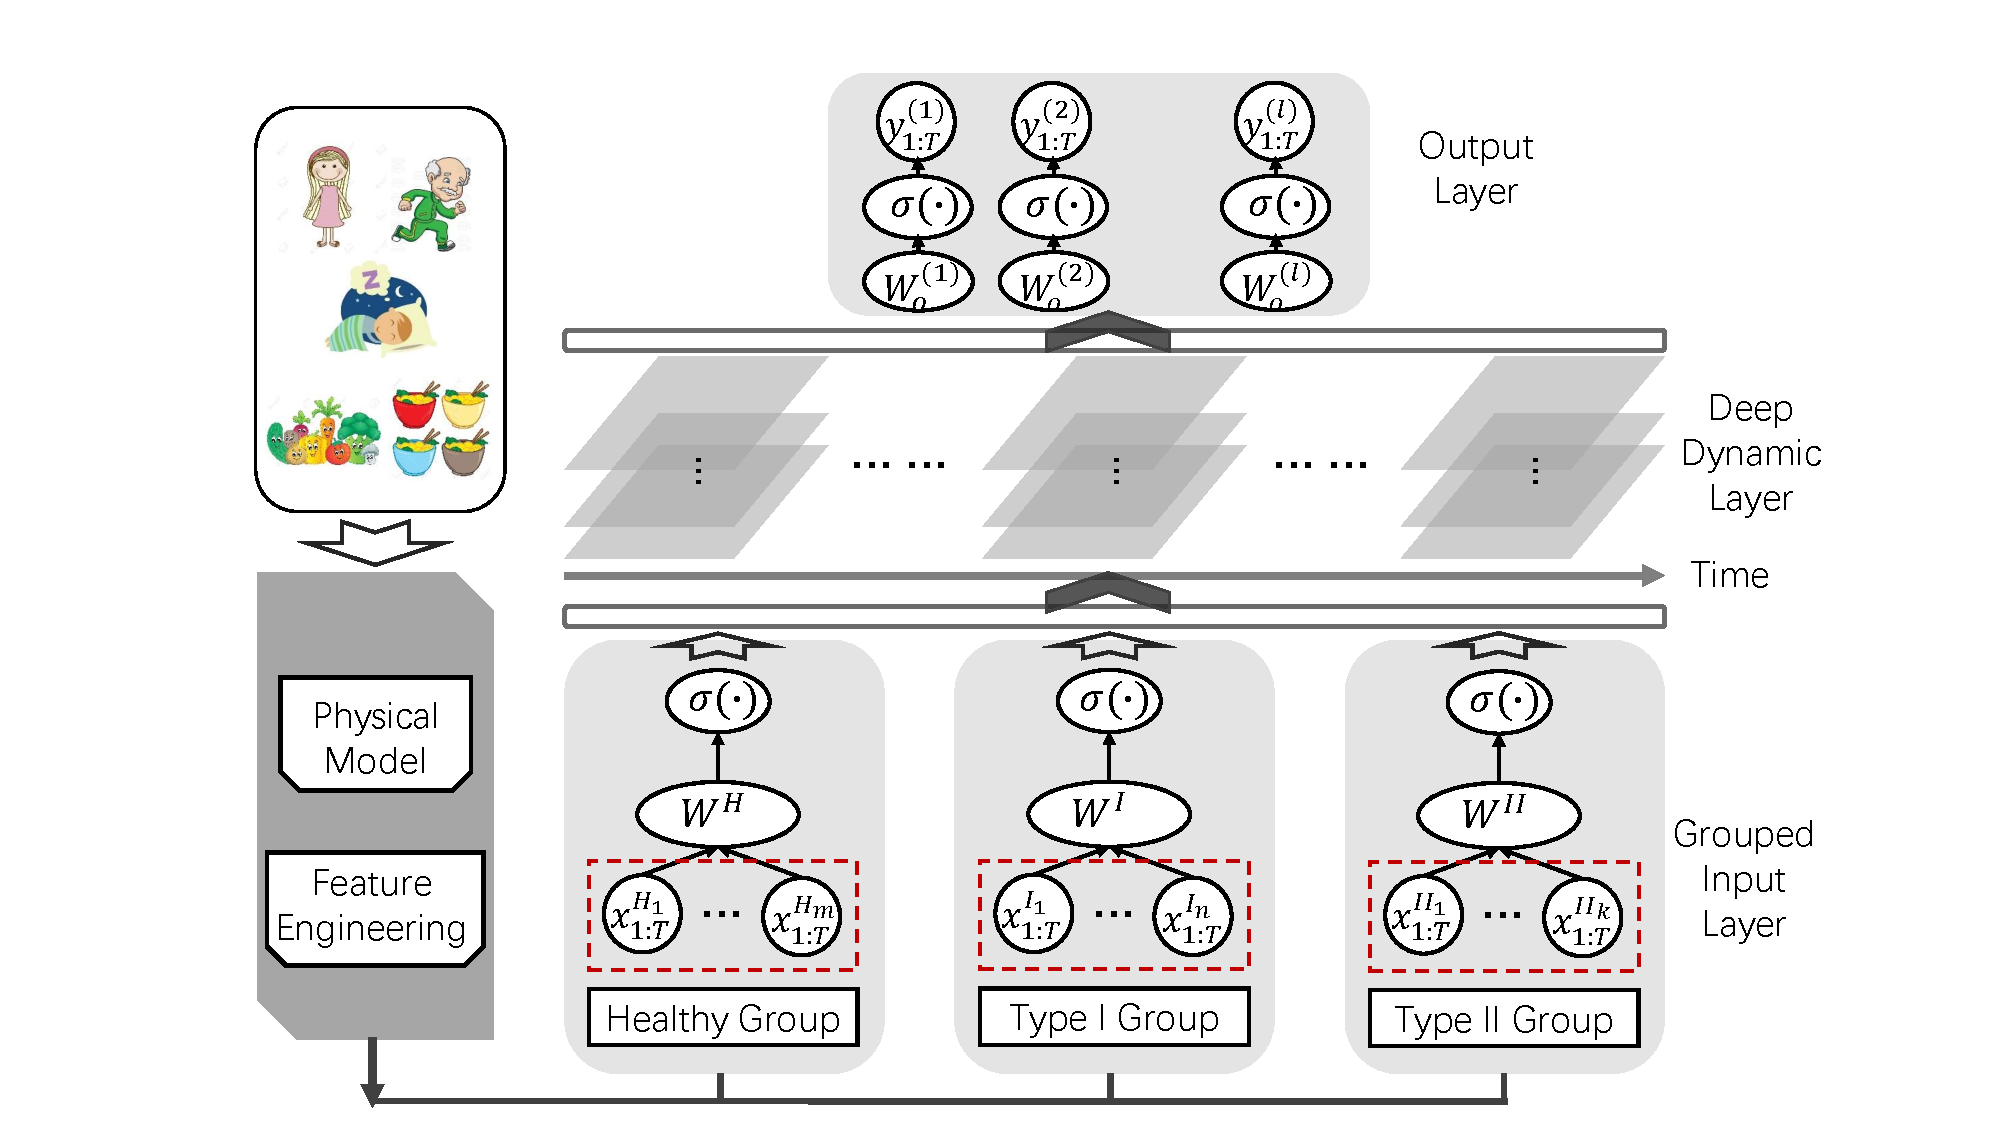
\includegraphics[width=0.9\columnwidth]{./img/pics_RNN.pdf}
  \caption{The Md$^3$RNN structure}
  \label{fig:rnn}
\end{figure}

\subsection{Model construction by layers}
The input of the Md$^3$RNN are the features extracted from the physiological model. The labeled data sequences for user number $j$ at time $t$ are denoted by $(x_i^{j},y_i^{j})$. We also adopt an index set convention, that $(x_A^{B},y_A^B)$ represents the data set $\left\{(x_i^{j},y_i^{j}) | i \in A, j\in B\right\}$ given index sets $A$ and $B$.
\subsubsection{Grouped Input Layer}
In the context of blood glucose prediction, available inputs are naturally divided into three groups according to the health condition of the participant from whom the data was generated. Notation-wise, we utilize $H$, $I$ and $II$ to indicate the the group of healthy user, user with type I diabetes and those having type II diabetes, respectively. Since the extracted features are essentially physiological indexes of an ``average'' person, they must go though different transformations to represent useful information of three distinct groups. This consideration motivate the design of the input layer (bottom of Fig.\ref{fig:rnn}) - it is divided into three units that performs different linear and non-linear transformation according to user groups. For instant, a data sample $x_t^{I_j}$, generated at time $t$ from the $j^{th}$ user of type I, undergoes the following processing:
\begin{align}
\tilde{x}_t^{I_j} = \sigma \left( W^Ix_t^{I_j} \right)
\end{align}     
where $W^I$ is the coefficients of the affine transformation \footnote{We assume that the interception is included in $W$. This can be done by simply adding a feature of all $1$s.}, $\sigma$ is some activation function, and $\tilde{x}_t^{I_j}$ is the output of the input layer for that data sample. Similar operations are conducted for data samples from group $H$ and $II$, but with different transformation coefficients. Intuitively, the shared transformation within groups would improve the learning of parameters (vs. single task learning), as information from all data in a homogeneous group is used.  

\subsubsection{Deep Dynamic Layer}
A common hidden layer is designated to capture the dynamics of the blood glucose evolution process. The underlying assumption is that, the biological and chemical reactions governing blood glucose variation are similar for all people, despite of grouped behaviors in the representation of physiological indexes (input layer), or individual characteristics in exhibited glucose level. This assumption could be justified by a series of medical research[][]. Moreover, since all users share the same hidden layer, all collected data samples are eventually helping the estimation of its parameters. The availability of rich information for the hidden layer makes the learning of a deep structure possible. In Md$^3$RNN, a number of Long Short Term Memory (LSTM) networks are stacked together (middle of Fig.\ref{fig:rnn}), to increase the overall model flexibility. In particular, it has been justified in both theory and practice that stacked LSTMs are able to capture dynamics occurring at different time scales, which in the current application would enable the modeling of both slow and rapid biological/chemical reactions. Mathematically, given the output from the grouped input layer, the deep dynamic layer performs
\begin{align}
h^0_t=
\end{align}



\subsubsection{Personalized Output Layer}


\subsection{Cost Sensitive Learning and Hyperparamter selection}